\providecommand{\main}{../../../..}
\documentclass[\main/dresen_thesis.tex]{subfiles}
\begin{document}
  \begin{figure}[tb]
    \centering
    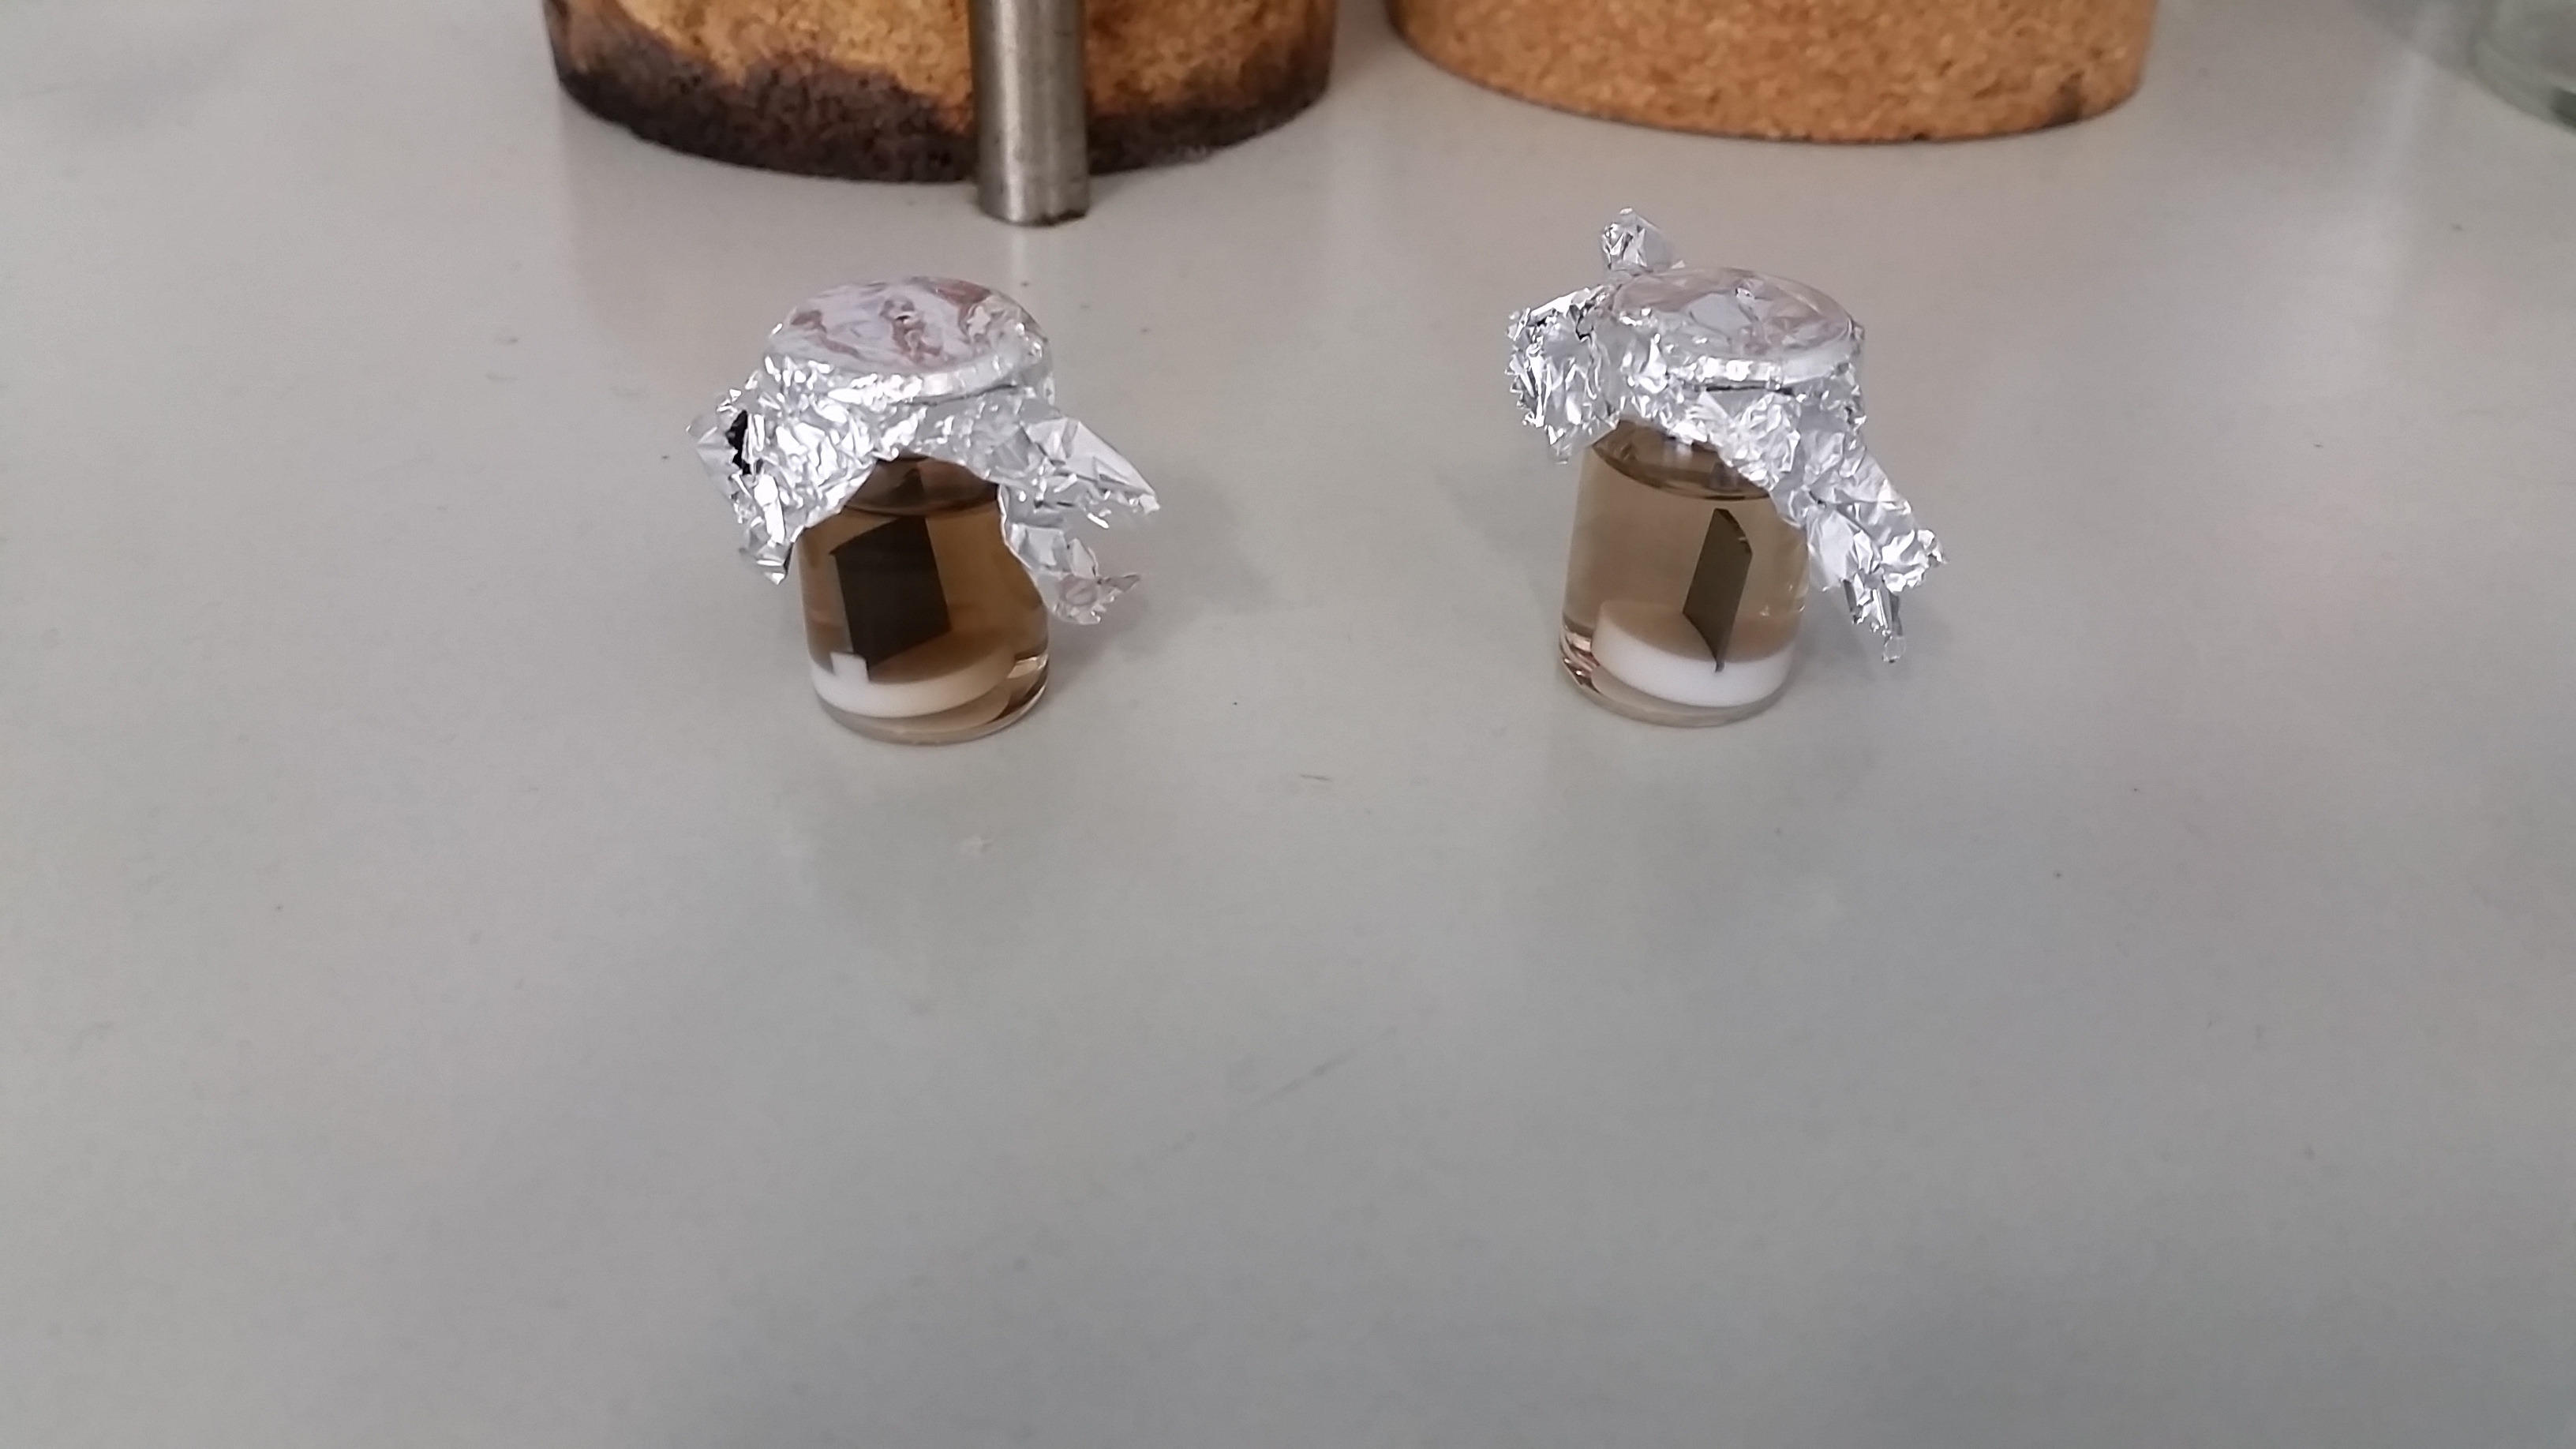
\includegraphics[width=0.79\textwidth]{colloidalCrystals_crystalPreparation}
    \caption{\label{fig:colloidalCrystals:preparation:image}Preparation of the colloidal crystals by the slow evaporation of a dispersion of nanoparticles.}
  \end{figure}

  \begin{table}[!htbp]
    \centering
    \caption{\label{tab:colloidalCrystals:preparation:conditions} Dispersion concentration used during the vertical drying.}
    \begin{tabular}{ l | l }
      \textbf{Sample}  & $c_m \, /  \unit{mg \, mL^{-1}}$\\
      \hline
      CC-Fe-0.25    & $0.25$\\
      CC-Fe-0.37    & $0.37$\\
      CC-Fe-0.50    & $0.50$\\
      \hline
    \end{tabular}
  \end{table}

  Write something
  % A quick and effective way to transfer nanoparticles from a dispersion to a homogeneously flat thin layer on a substrate is spin coating.
  % Here, a droplet of a dispersion with a high concentration of nanoparticles is transferred on a substrate, which is subsequently rotated with a high angular frequency.
  % Due to the centrifugal force, most parts of the dispersion is removed from the substrate and only a homogeneous thin layer remains on the substrate.
  % The thickness of the thin nanoparticle layer can be tuned by variation of the rotation speed, the nanoparticle concentration in dispersion, and the time that the substrate is rotated.
  % On the one hand spin coating produces quickly and effectively thin layers with homogeneous thickness, but on the other hand it is highly inefficient in material usage, as most parts are lost during the process.

  % Thin layer samples discussed in this chapter were prepared by the same collaboration that produced the nanoparticles.
  % As substrate, silicon wafers were chosen and pretreated for 30 minutes in a fresh Piranha solution (\ch{H2SO4} [conc.] and \ch{H2O2} [30\%] in a ratio of 2:1). Subsequently, they were washed with \ch{EtOH}, dried in a nitrogen stream and heated in an oven to $450 ^\circ \mathrm{C}$ for one hour.
  % After that procedures any organic remain is removed from the silicon and the nanoparticle dispersion in $\mathit{n}$-hexane is spin coated on the substrate.

  % More complex samples are prepared by subsequently spin-coating layers of PMMA and nanoparticles on a substrate.
  % Two samples were prepared for each nanoparticle batch with varied PMMA concentration to vary the thickness of the PMMA layer.
  % The PMMA is dispersed in ethyl acetate and for each sample, the spin-coating process is started with a PMMA layer.
  % After each spin-coating, the sample is baked at $120 \unit{^\circ C}$ for $20 \unit{min}$ to remove any remaining solvent.
  % In total, eight bilayers of PMMA/nanoparticles were spin coated for all four samples.
\end{document}